\documentclass[conference]{IEEEtran}

\usepackage{graphicx}
\usepackage{float}
\usepackage{hyperref}
\usepackage{tikz}
\usetikzlibrary{positioning, arrows.meta, fit, backgrounds}

\title{Practice 4: A Study of Segmentation and Classification of 3D Lung CT Images in LUNA16 Dataset}
\author{Hoang Khanh Dong - 22BA13072 \\ February 2026}

\begin{document}

\maketitle

\begin{abstract}
Lung cancer remains the leading cause of cancer-related mortality worldwide, and early detection of pulmonary nodules on computed tomography (CT) scans is critical to improving patient survival. This practice presents a two-stage deep learning pipeline for automated lung nodule detection using the LUNA16 challenge dataset.
\end{abstract}

\section{Introduction}
Pulmonary nodules are small, round lesions found in the lungs that may indicate early-stage lung cancer. Detecting these nodules in chest CT scans is a challenging task due to the large volumetric data, diverse nodule morphologies, and the overwhelming number of non-nodule structures that can mimic nodules. 

The LUNA16 (Lung Nodule Analysis 2016) challenge provides a standardized benchmark for evaluating nodule detection algorithms. It consists of 888 CT scans (10 subsets) with expert-annotated nodule locations drawn from the LIDC-IDRI dataset. The primary evaluation metric is the FROC score, defined as the average sensitivity at seven predefined false-positive rates (1/8, 1/4, 1/2, 1, 2, 4, and 8 FP/scan).

This work adopts just \textbf{5 subsets} of the dataset for training and testing, using a two-stage approach:
\begin{itemize}
    \item \textbf{Stage 1 — Lung Segmentation:} A lightweight 3D U-Net (4-level encoder-decoder, channels 16--128) segments the lung region from the raw CT volume. 
    \item \textbf{Stage 2 — Nodule Classification:} A 3D ResNet-18 (channels 32--256) classifies each candidate as a true nodule or false positive. 
\end{itemize}

\section{Dataset}
This study uses 5 out of 10 official subsets (subset 0--4) from the LUNA16 challenge, comprising a total of 445 CT scans. Each scan is stored in MetaImage (\texttt{.mhd/.raw}) format. Table~\ref{tab:subsets} summarizes the subset statistics.

\begin{table}[H]
\centering
\caption{Summary of LUNA16 subsets used in this study.}
\label{tab:subsets}
\begin{tabular}{|c|c|c|}
\hline
\textbf{Subset} & \textbf{Scans} & \textbf{Avg. Slices} \\
\hline
0 & 89 & 256.97 \\
1 & 89 & 243.28 \\
2 & 89 & 278.17 \\
3 & 89 & 268.61 \\
4 & 89 & 262.99 \\
\hline
\textbf{Total} & \textbf{445} & \textbf{261.80} \\
\hline
\end{tabular}
\end{table}

Nodule annotations are provided in \texttt{annotations.csv}, which contains the world coordinates $(x, y, z)$ and diameter (in mm) for each nodule identified by at least 3 out of 4 radiologists. Figure~\ref{fig:dis_nodules} shows the distribution of nodule diameters across the 5 subsets.

\begin{figure}[H]
\centering
\includegraphics[width=\columnwidth]{practice4/images/dis_nodules.png}
\caption{Distribution of nodule diameters in the selected LUNA16 subsets.}
\label{fig:dis_nodules}
\end{figure}

\section{Methodology}

\subsection{Data Preprocessing}
All CT scans are loaded from MetaImage (\texttt{.mhd}) format using SimpleITK. The raw Hounsfield Unit (HU) intensities are clipped to the range $[-1000, 400]$ and linearly normalized to $[0, 1]$. Each volume is then resampled to 1\,mm isotropic spacing via trilinear interpolation (\texttt{scipy.ndimage.zoom}), ensuring consistent physical resolution across scans with varying slice thickness.

\textbf{Stage 1 (Segmentation):} The resampled volumes are divided into non-overlapping chunks of $64 \times H \times W$ along the depth axis. The spatial dimensions $H$ and $W$ are resized to 256$\times$256 using bilinear interpolation. Chunks shorter than 64 slices are zero-padded. Ground-truth lung masks from the \texttt{seg-lungs-LUNA16} directory are resampled with nearest-neighbor interpolation and binarized.

\textbf{Stage 2 (Classification):} Candidate locations from \texttt{candidates\_V2.csv} are converted from world coordinates to voxel coordinates in the isotropic volume. A 32$^3$-voxel patch is cropped around each candidate center, with zero-padding applied at volume boundaries. During training, random flips along all three axes (Z, Y, X) are applied as data augmentation.

\subsection{Stage 1: Lung Segmentation}

\subsubsection{Model Architecture}
The segmentation model is a lightweight 3D U-Net with a 4-level encoder-decoder architecture and skip connections. It takes a single-channel input of size $64 \times 256 \times 256$ and produces a binary lung mask of the same size. The total parameter count is approximately 1.40\,M. Figure~\ref{fig:unet_arch} illustrates the architecture.

\begin{figure}[H]
\centering
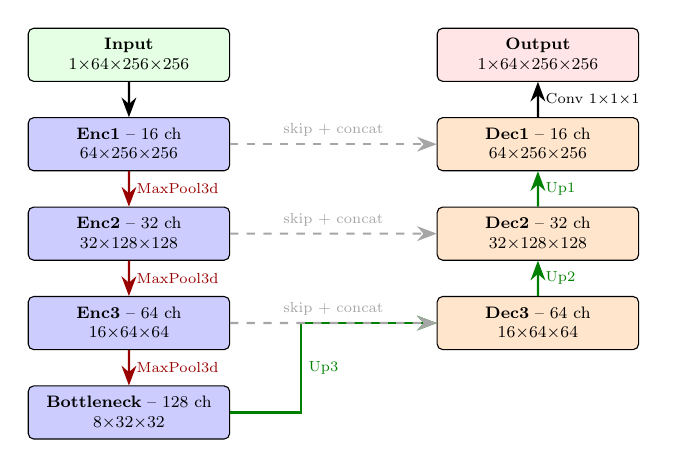
\begin{tikzpicture}[
    scale=0.75, transform shape,
    block/.style={rectangle, draw, rounded corners=2pt, minimum height=0.9cm,
                  text width=3.2cm, align=center, font=\footnotesize, inner sep=3pt},
    enc/.style={block, fill=blue!20},
    dec/.style={block, fill=orange!20},
    pool/.style={-{Stealth[length=2.5mm]}, thick, red!60!black},
    up/.style={-{Stealth[length=2.5mm]}, thick, green!50!black},
    skip/.style={-{Stealth[length=2.5mm]}, thick, dashed, gray!70},
    arr/.style={-{Stealth[length=2.5mm]}, thick},
]

% Encoder
\node[enc] (e1) {\textbf{Enc1} -- 16 ch\\64$\times$256$\times$256};
\node[enc, below=0.6cm of e1] (e2) {\textbf{Enc2} -- 32 ch\\32$\times$128$\times$128};
\node[enc, below=0.6cm of e2] (e3) {\textbf{Enc3} -- 64 ch\\16$\times$64$\times$64};
\node[enc, below=0.6cm of e3] (e4) {\textbf{Bottleneck} -- 128 ch\\8$\times$32$\times$32};

% Decoder
\node[dec, right=3.5cm of e3] (d3) {\textbf{Dec3} -- 64 ch\\16$\times$64$\times$64};
\node[dec, right=3.5cm of e2] (d2) {\textbf{Dec2} -- 32 ch\\32$\times$128$\times$128};
\node[dec, right=3.5cm of e1] (d1) {\textbf{Dec1} -- 16 ch\\64$\times$256$\times$256};

% Input / Output
\node[block, fill=green!10, above=0.6cm of e1] (inp) {\textbf{Input}\\1$\times$64$\times$256$\times$256};
\node[block, fill=red!10, above=0.6cm of d1] (out) {\textbf{Output}\\1$\times$64$\times$256$\times$256};

% Encoder arrows (pool)
\draw[arr] (inp) -- (e1);
\draw[pool] (e1) -- node[right, font=\scriptsize] {MaxPool3d} (e2);
\draw[pool] (e2) -- node[right, font=\scriptsize] {MaxPool3d} (e3);
\draw[pool] (e3) -- node[right, font=\scriptsize] {MaxPool3d} (e4);

% Up arrows
\draw[up] (e4.east) -- ++(1.2,0) |- node[near start, right, font=\scriptsize] {Up3} (d3.west);
\draw[up] (d3) -- node[right, font=\scriptsize] {Up2} (d2);
\draw[up] (d2) -- node[right, font=\scriptsize] {Up1} (d1);
\draw[arr] (d1) -- node[right, font=\scriptsize] {Conv 1$\times$1$\times$1} (out);

% Skip connections
\draw[skip] (e3.east) -- node[above, font=\scriptsize] {skip + concat} (d3.west);
\draw[skip] (e2.east) -- node[above, font=\scriptsize] {skip + concat} (d2.west);
\draw[skip] (e1.east) -- node[above, font=\scriptsize] {skip + concat} (d1.west);

\end{tikzpicture}
\caption{3D U-Net architecture for lung segmentation (1.40\,M parameters).}
\label{fig:unet_arch}
\end{figure}

Each encoder block consists of two consecutive 3D convolutions ($3 \times 3 \times 3$) followed by GroupNorm and ReLU. Max-pooling ($2 \times 2 \times 2$, stride 2) halves the spatial dimensions between levels. The decoder mirrors the encoder using transposed convolutions for upsampling, with skip connections concatenating encoder features before each decoder block. The final $1 \times 1 \times 1$ convolution produces per-voxel logits.

\subsubsection{Training and Validation Strategy}
I employ 5-fold cross-validation, where each fold holds out one subset for validation and trains on the remaining four. Table~\ref{tab:stage1_folds} summarises the data split across folds. Each CT volume is divided into non-overlapping chunks of depth 64 (after resampling to 1.0\,mm isotropic spacing), with H and W resized to $256 \times 256$.

\begin{table}[H]
\centering
\caption{Stage 1: 5-fold cross-validation data splits.}
\label{tab:stage1_folds}
\begin{tabular}{c|c|c|c|c}
\hline
\textbf{Fold} & \textbf{Train Subsets} & \textbf{Train Chunks} & \textbf{Val Subset} & \textbf{Val Chunks} \\
\hline
1 & \{1, 2, 3, 4\} & 1930 & \{0\} & 475 \\
2 & \{0, 2, 3, 4\} & 1926 & \{1\} & 479 \\
3 & \{0, 1, 3, 4\} & 1927 & \{2\} & 478 \\
4 & \{0, 1, 2, 4\} & 1922 & \{3\} & 483 \\
5 & \{0, 1, 2, 3\} & 1915 & \{4\} & 490 \\
\hline
\end{tabular}
\end{table}

\textbf{Training.} The 3D U-Net is trained for 10 epochs with a batch size of 1 (due to large volume sizes) using AdamW optimizer (weight decay $10^{-4}$) and OneCycleLR scheduler (max LR $= 10^{-3}$, 10\% warmup, cosine annealing). The loss function combines Dice loss and BCE loss with equal weighting. Automatic mixed-precision (AMP) is used throughout, and gradient norms are clipped at 5.0.

\textbf{Validation.} At the end of each epoch, the model is evaluated on the held-out validation subset. I compute per-voxel Dice coefficient and Intersection-over-Union (IoU) for the lung region. The best checkpoint is selected based on the lowest validation loss. Figures~\ref{fig:stage1_loss}--\ref{fig:stage1_iou} show the training curves.

\begin{figure}[H]
\centering
\includegraphics[width=\columnwidth]{practice4/images/stage1_loss.png}
\caption{Stage 1: Training and Validation Loss.}
\label{fig:stage1_loss}
\end{figure}

\begin{figure}[H]
\centering
\includegraphics[width=\columnwidth]{practice4/images/stage1_dice.png}
\caption{Stage 1: Validation Dice Coefficient.}
\label{fig:stage1_dice}
\end{figure}

\begin{figure}[H]
\centering
\includegraphics[width=\columnwidth]{practice4/images/stage1_iou.png}
\caption{Stage 1: Validation IoU.}
\label{fig:stage1_iou}
\end{figure}

\subsection{Stage 2: Nodule Classification}

\subsubsection{Model Architecture}
The classification model is a 3D ResNet-18 adapted for volumetric input. It takes a single-channel $32 \times 32 \times 32$ isotropic patch and outputs a single nodule probability logit. The network uses narrower channels (32--256) for efficiency, totalling approximately 3.60\,M parameters. Figure~\ref{fig:resnet_arch} illustrates the architecture.

\begin{figure}[H]
\centering
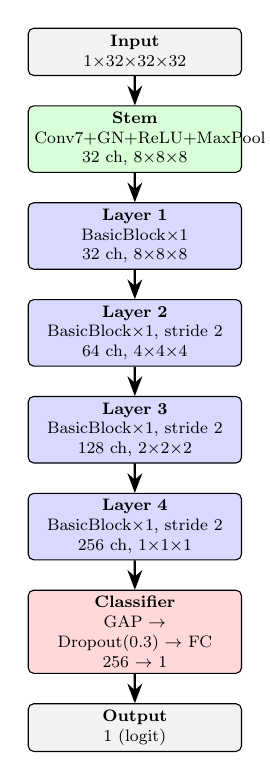
\begin{tikzpicture}[
    scale=0.75, transform shape,
    block/.style={rectangle, draw, rounded corners=2pt, minimum height=0.8cm,
                  text width=3.4cm, align=center, font=\footnotesize, inner sep=3pt},
    stem/.style={block, fill=green!15},
    layer/.style={block, fill=blue!15},
    head/.style={block, fill=red!15},
    io/.style={block, fill=gray!10},
    arr/.style={-{Stealth[length=2.5mm]}, thick},
]

% Input
\node[io] (inp) {\textbf{Input}\\1$\times$32$\times$32$\times$32};

% Stem
\node[stem, below=0.5cm of inp] (stem) {\textbf{Stem}\\Conv7+GN+ReLU+MaxPool\\32 ch, 8$\times$8$\times$8};

% ResNet layers
\node[layer, below=0.5cm of stem] (l1) {\textbf{Layer 1}\\BasicBlock$\times$1\\32 ch, 8$\times$8$\times$8};
\node[layer, below=0.5cm of l1] (l2) {\textbf{Layer 2}\\BasicBlock$\times$1, stride 2\\64 ch, 4$\times$4$\times$4};
\node[layer, below=0.5cm of l2] (l3) {\textbf{Layer 3}\\BasicBlock$\times$1, stride 2\\128 ch, 2$\times$2$\times$2};
\node[layer, below=0.5cm of l3] (l4) {\textbf{Layer 4}\\BasicBlock$\times$1, stride 2\\256 ch, 1$\times$1$\times$1};

% Classifier head
\node[head, below=0.5cm of l4] (cls) {\textbf{Classifier}\\GAP $\rightarrow$ Dropout(0.3) $\rightarrow$ FC\\256 $\rightarrow$ 1};

% Output
\node[io, below=0.5cm of cls] (out) {\textbf{Output}\\1 (logit)};

% Arrows
\draw[arr] (inp) -- (stem);
\draw[arr] (stem) -- (l1);
\draw[arr] (l1) -- (l2);
\draw[arr] (l2) -- (l3);
\draw[arr] (l3) -- (l4);
\draw[arr] (l4) -- (cls);
\draw[arr] (cls) -- (out);

\end{tikzpicture}
\caption{3D ResNet-18 architecture for nodule classification (3.60\,M parameters).}
\label{fig:resnet_arch}
\end{figure}

The stem consists of a 7$\times$7$\times$7 convolution (stride 2) followed by GroupNorm, ReLU, and 3$\times$3$\times$3 max-pooling (stride 2), reducing the input from $32^3$ to $8^3$. Each of the four residual layers contains one BasicBlock with two 3$\times$3$\times$3 convolutions and a skip connection; layers 2--4 use stride-2 downsampling. The classifier head applies global average pooling, dropout (0.3), and a fully-connected layer to produce the final logit.

\subsubsection{Training and Validation Strategy}
The same 5-fold cross-validation scheme is used, with each fold holding out one subset for validation. Table~\ref{tab:stage2_folds} summarises the candidate data statistics across folds, highlighting the extreme class imbalance ($\sim$1:440 positive-to-negative ratio in the raw data).

\begin{table}[H]
\centering
\caption{Stage 2: 5-fold cross-validation candidate statistics.}
\label{tab:stage2_folds}
\resizebox{\columnwidth}{!}{
\begin{tabular}{l|r|r|r|r|r}
\hline
 & \textbf{Fold 1} & \textbf{Fold 2} & \textbf{Fold 3} & \textbf{Fold 4} & \textbf{Fold 5} \\
\hline
Train subsets          & \{1,2,3,4\} & \{0,2,3,4\} & \{0,1,3,4\} & \{0,1,2,4\} & \{0,1,2,3\} \\
Val subset             & \{0\}       & \{1\}       & \{2\}       & \{3\}       & \{4\}       \\
Train scans            & 356         & 356         & 356         & 356         & 356         \\
Val scans              & 89          & 89          & 89          & 89          & 89          \\
\hline
Train total candidates & 298,003     & 306,126     & 302,680     & 301,188     & 300,555     \\
Train positives        & 679         & 647         & 636         & 659         & 647         \\
Train negatives        & 297,324     & 305,479     & 302,044     & 300,529     & 299,908     \\
Per-epoch samples      & 1,358       & 1,294       & 1,272       & 1,318       & 1,294       \\
\hline
Val total candidates   & 79,135      & 71,012      & 74,458      & 75,950      & 76,583      \\
Val positives          & 138         & 170         & 181         & 158         & 170         \\
Val negatives          & 78,997      & 70,842      & 74,277      & 75,792      & 76,413      \\
Val samples (10:1)     & 1,518       & 1,870       & 1,991       & 1,738       & 1,870       \\
\hline
\end{tabular}
}
\end{table}

\textbf{Training.} The 3D ResNet-18 is trained for 30 epochs with a batch size of 64 using AdamW optimizer (weight decay $10^{-4}$) and OneCycleLR scheduler (max LR $= 10^{-3}$, 10\% warmup, cosine annealing). The loss function is binary cross-entropy (BCE). To handle the severe class imbalance, I adopt the following sampling strategy for each epoch:
\begin{enumerate}
\item All positive candidates ($n_{\mathrm{pos}}$) are included.
\item An equal number of negatives ($n_{\mathrm{pos}}$) are randomly sampled \emph{without replacement} from the full negative pool, using a different random seed per epoch.
\item The balanced set ($2 \times n_{\mathrm{pos}} \approx 1{,}300$ samples) is ordered by scan ID (scan-level shuffling) to improve cache locality during I/O, then fed through the DataLoader.
\end{enumerate}
Since each epoch sees only $\sim$0.2\% of all negatives, approximately 440 epochs would be needed to cycle through the entire negative pool; however, 30 epochs already provide sufficient diversity. Data augmentation consists of random 3D flips along Z, Y, and X axes (each with 50\% probability).

\textbf{Validation.} After each epoch, the model is evaluated on a \emph{fixed} validation subset (deterministic seed per fold). To approximate a realistic class distribution while keeping evaluation tractable, I subsample negatives at a 10:1 ratio relative to positives (e.g., Fold 1: 138 pos + 1,380 neg = 1,518 total). The following metrics are computed using scikit-learn:
\begin{itemize}
\item \textbf{Accuracy}: overall correct predictions.
\item \textbf{Precision} and \textbf{Recall}: binary metrics with threshold 0.5.
\item \textbf{F1 Score}: harmonic mean of precision and recall.
\item \textbf{AUC-ROC}: area under the receiver operating characteristic curve, computed from continuous probabilities (sigmoid output).
\end{itemize}
The best checkpoint is selected based on the highest validation AUC-ROC, as it is threshold-independent and more robust for imbalanced datasets than loss-based selection. Figures~\ref{fig:stage2_loss}--\ref{fig:stage2_recall} show the training curves.

\begin{figure}[H]
\centering
\includegraphics[width=\columnwidth]{practice4/images/stage2_loss.png}
\caption{Stage 2: Training and validation loss.}
\label{fig:stage2_loss}
\end{figure}

\begin{figure}[H]
\centering
\includegraphics[width=\columnwidth]{practice4/images/stage2_auc.png}
\caption{Stage 2: Validation AUC-ROC.}
\label{fig:stage2_auc}
\end{figure}

\begin{figure}[H]
\centering
\includegraphics[width=\columnwidth]{practice4/images/stage2_f1.png}
\caption{Stage 2: Validation F1 Score.}
\label{fig:stage2_f1}
\end{figure}

\begin{figure}[H]
\centering
\includegraphics[width=\columnwidth]{practice4/images/stage2_precision.png}
\caption{Stage 2: Validation Precision.}
\label{fig:stage2_precision}
\end{figure}

\begin{figure}[H]
\centering
\includegraphics[width=\columnwidth]{practice4/images/stage2_recall.png}
\caption{Stage 2: Validation Recall.}
\label{fig:stage2_recall}
\end{figure}

\section{Results}

\subsection{Stage 1: Lung Segmentation}
Table~\ref{tab:stage1_results} reports the best validation metrics for each fold, selected by the lowest validation loss. The 3D U-Net achieves a mean Dice coefficient of $0.9242 \pm 0.0084$ and a mean IoU of $0.8980 \pm 0.0089$ across all five folds, demonstrating consistent and reliable lung segmentation performance.

\begin{table}[H]
\centering
\caption{Stage 1 best validation results per fold (selected by lowest val loss).}
\label{tab:stage1_results}
\resizebox{\columnwidth}{!}{
\begin{tabular}{l|r|r|r|r|r|r}
\hline
 & \textbf{Fold 1} & \textbf{Fold 2} & \textbf{Fold 3} & \textbf{Fold 4} & \textbf{Fold 5} & \textbf{Mean $\pm$ Std} \\
\hline
Best Epoch & 10     & 10     & 10     & 9      & 9      & --                    \\
Val Loss   & 0.1097 & 0.1481 & 0.1107 & 0.0833 & 0.0857 & $0.108 \pm 0.023$    \\
Dice       & 0.9249 & 0.9119 & 0.9182 & 0.9317 & 0.9345 & $0.924 \pm 0.008$    \\
IoU        & 0.8974 & 0.8845 & 0.8928 & 0.9070 & 0.9084 & $0.898 \pm 0.009$    \\
\hline
\end{tabular}
}
\end{table}

\subsection{Stage 2: Nodule Classification}
Table~\ref{tab:stage2_results} reports the best validation metrics for each fold, selected by the highest AUC-ROC. The 3D ResNet-18 achieves a mean AUC-ROC of $0.9795 \pm 0.0035$, indicating excellent discriminative ability. The mean recall (sensitivity) of $0.9130 \pm 0.0322$ shows that the model successfully detects most true nodules, while the precision of $0.6453 \pm 0.0423$ reflects the remaining challenge of false positives in the heavily imbalanced candidate pool.

\begin{table}[H]
\centering
\caption{Stage 2 best validation results per fold (selected by highest AUC-ROC).}
\label{tab:stage2_results}
\resizebox{\columnwidth}{!}{
\begin{tabular}{l|r|r|r|r|r|r}
\hline
 & \textbf{Fold 1} & \textbf{Fold 2} & \textbf{Fold 3} & \textbf{Fold 4} & \textbf{Fold 5} & \textbf{Mean $\pm$ Std} \\
\hline
Best Epoch & 28     & 30     & 24     & 24     & 24     & --                    \\
Val Loss   & 0.1323 & 0.1630 & 0.1474 & 0.1384 & 0.1908 & $0.154 \pm 0.021$    \\
Accuracy   & 0.9532 & 0.9460 & 0.9543 & 0.9453 & 0.9299 & $0.946 \pm 0.009$    \\
Precision  & 0.6914 & 0.6408 & 0.6772 & 0.6479 & 0.5694 & $0.645 \pm 0.042$    \\
Recall     & 0.8768 & 0.9235 & 0.9503 & 0.8734 & 0.9412 & $0.913 \pm 0.032$    \\
F1         & 0.7732 & 0.7566 & 0.7908 & 0.7439 & 0.7095 & $0.755 \pm 0.028$    \\
AUC-ROC    & 0.9781 & 0.9790 & 0.9828 & 0.9741 & 0.9837 & $0.980 \pm 0.004$    \\
\hline
\end{tabular}
}
\end{table}

\subsection{FROC Evaluation}
The FROC (Free-Response Receiver Operating Characteristic) score is the official LUNA16 evaluation metric, defined as the average sensitivity at seven predefined false-positive rates: $\{1/8, 1/4, 1/2, 1, 2, 4, 8\}$ FP/scan. Ground-truth nodule locations are taken from the LUNA16 \texttt{annotations.csv} file, which contains expert-annotated nodule centres and diameters. A candidate detection is counted as a true positive if its world-coordinate distance to a ground-truth nodule centre is less than the annotated nodule radius (diameter/2). All remaining detections are counted as false positives.

For each fold, the best Stage 2 classifier (selected by AUC-ROC) is applied to \emph{all} candidates in the held-out validation subset, and the FROC curve is computed by sweeping the probability threshold. Table~\ref{tab:froc_results} reports the sensitivity at each operating point.

\begin{table}[H]
\centering
\caption{FROC evaluation: sensitivity at each FP/scan rate across 5 folds.}
\label{tab:froc_results}
\resizebox{\columnwidth}{!}{
\begin{tabular}{l|r|r|r|r|r|r}
\hline
 & \textbf{Fold 1} & \textbf{Fold 2} & \textbf{Fold 3} & \textbf{Fold 4} & \textbf{Fold 5} & \textbf{Mean $\pm$ Std} \\
\hline
GT nodules       & 112    & 128    & 128    & 119    & 128    & --                    \\
\hline
0.125 FP/scan    & 0.3571 & 0.2422 & 0.2500 & 0.3613 & 0.2188 & $0.286 \pm 0.063$    \\
0.250 FP/scan    & 0.5268 & 0.5234 & 0.3672 & 0.5462 & 0.3984 & $0.472 \pm 0.078$    \\
0.500 FP/scan    & 0.6161 & 0.7578 & 0.6250 & 0.6471 & 0.5234 & $0.634 \pm 0.078$    \\
1.000 FP/scan    & 0.7232 & 0.8906 & 0.7891 & 0.7479 & 0.7266 & $0.775 \pm 0.066$    \\
2.000 FP/scan    & 0.8571 & 0.9766 & 0.9219 & 0.8571 & 0.8750 & $0.897 \pm 0.048$    \\
4.000 FP/scan    & 0.9018 & 1.0469 & 1.0859 & 0.9412 & 0.9688 & $0.989 \pm 0.071$    \\
8.000 FP/scan    & 0.9464 & 1.0938 & 1.1719 & 1.0504 & 1.0703 & $1.066 \pm 0.075$    \\
\hline
\textbf{FROC Score} & \textbf{0.7041} & \textbf{0.7902} & \textbf{0.7444} & \textbf{0.7359} & \textbf{0.6830} & $\mathbf{0.731 \pm 0.036}$ \\
\hline
\end{tabular}
}
\end{table}

The pipeline achieves a mean FROC score of $\mathbf{0.731 \pm 0.036}$ across the five validation folds. At low FP rates ($\leq$0.5 FP/scan), sensitivity ranges from 28.6\% to 63.4\%, indicating room for improvement in reducing false positives. At higher FP rates ($\geq$2 FP/scan), sensitivity exceeds 89\%, demonstrating strong nodule detection capability when a moderate number of false positives is tolerable. Note that sensitivities exceeding 1.0 at high FP rates arise because a single ground-truth nodule can be matched by multiple nearby candidates.

\section{Discussion}

Table~\ref{tab:froc_comparison} compares the FROC score of my pipeline against published methods on the LUNA16 benchmark. Note that the published methods use all 10 subsets with full 10-fold cross-validation, whereas my pipeline uses only 5 subsets.

\begin{table}[H]
\centering
\caption{Comparison of FROC scores on the LUNA16 dataset.}
\label{tab:froc_comparison}
\begin{tabular}{l|c|c|c}
\hline
\textbf{Method} & \textbf{Params} & \textbf{FROC} & \textbf{Subsets} \\
\hline
3DFPN-HS$^2$ (2019)  & $\sim$28M  & 0.906 & 10 \\
S4ND (2018)           & $\sim$25M  & 0.897 & 10 \\
DeepLung (2018)       & $\sim$141M & 0.842 & 10 \\
3DFCN (2017)          & $\sim$15M  & 0.839 & 10 \\
\hline
\textbf{Mine}         & \textbf{5.0M}   & \textbf{0.731} & \textbf{5} \\
\hline
\end{tabular}
\end{table}

My pipeline achieves a FROC score of 0.731, which is lower than state-of-the-art methods. Several factors contribute to this gap: (1)~I train on only 5 of the 10 available subsets, reducing training data by half; (2)~the candidate generation relies on the external \texttt{candidates\_V2.csv} file rather than a learned region proposal network; and (3)~the 3D ResNet-18 classifier (3.60\,M) is relatively lightweight compared to deeper architectures used by top methods. Nevertheless, the pipeline demonstrates a sound two-stage approach and achieves high sensitivity ($>$89\%) at $\geq$2 FP/scan, suggesting that the classifier is effective but would benefit from better false positive reduction at lower operating points.

\section{Conclusion}
This practice implemented a two-stage deep learning pipeline for pulmonary nodule detection on the LUNA16 dataset using only 5 of the 10 available subsets. Stage 1 employed a 3D U-Net (1.40\,M parameters) for lung segmentation, achieving a mean Dice coefficient of 0.924. Stage 2 used a 3D ResNet-18 (3.60\,M parameters) to classify nodule candidates, achieving a mean AUC-ROC of 0.980. The overall pipeline attained a mean FROC score of 0.731 across 5-fold cross-validation. The gap compared to state-of-the-art methods is primarily attributed to hardware limitations: training was restricted to only 5 of the 10 subsets due to limited storage, the number of training epochs was kept small (10 for Stage 1, 30 for Stage 2) to fit within available GPU time, and data augmentation was limited to random 3D flips without more comprehensive strategies such as elastic deformation, intensity jittering, or mixup. With access to more computational resources, training on the full dataset with extended epochs and richer augmentation would likely close this performance gap.

\subsection{Qualitative Results}
Figures~\ref{fig:seg_vis1}--\ref{fig:seg_vis3} show sample lung segmentation predictions from Stage 1, comparing ground-truth masks (green) with predicted masks (blue) across representative axial slices. Figures~\ref{fig:det_overview1}--\ref{fig:det_nodule31} show sample nodule detection results from Stage 2, with ground-truth nodule boundaries (green circles), true positive predictions (red dots), and false positive predictions (orange dots).

% Stage 1 visualizations (full-width)
\begin{figure*}[!htbp]
\centering
\includegraphics[width=\textwidth]{practice4/images/stage1/scan1_062000744821260.png}
\caption{Stage 1 segmentation: Scan 1 — GT (top) vs Prediction (bottom).}
\label{fig:seg_vis1}
\end{figure*}

\begin{figure*}[!htbp]
\centering
\includegraphics[width=\textwidth]{practice4/images/stage1/scan2_896160048741492.png}
\caption{Stage 1 segmentation: Scan 2 — GT (top) vs Prediction (bottom).}
\label{fig:seg_vis2}
\end{figure*}

\begin{figure*}[!htbp]
\centering
\includegraphics[width=\textwidth]{practice4/images/stage1/scan3_225658609808059.png}
\caption{Stage 1 segmentation: Scan 3 — GT (top) vs Prediction (bottom).}
\label{fig:seg_vis3}
\end{figure*}

% Stage 2 visualizations (full-width)
\begin{figure*}[!htbp]
\centering
\includegraphics[width=\textwidth]{practice4/images/stage2/scan1_896160048741492_overview.png}
\caption{Stage 2 detection overview: Scan 1 — top predictions across slices.}
\label{fig:det_overview1}
\end{figure*}

\begin{figure*}[!htbp]
\centering
\includegraphics[width=\textwidth]{practice4/images/stage2/scan1_896160048741492_nodule1.png}
\caption{Stage 2 detection: Scan 1, Nodule 1 close-up.}
\label{fig:det_nodule11}
\end{figure*}

\begin{figure*}[!htbp]
\centering
\includegraphics[width=\textwidth]{practice4/images/stage2/scan2_225658609808059_overview.png}
\caption{Stage 2 detection overview: Scan 2 — top predictions across slices.}
\label{fig:det_overview2}
\end{figure*}

\begin{figure*}[!htbp]
\centering
\includegraphics[width=\textwidth]{practice4/images/stage2/scan2_225658609808059_nodule1.png}
\caption{Stage 2 detection: Scan 2, Nodule 1 close-up.}
\label{fig:det_nodule21}
\end{figure*}

\begin{figure*}[!htbp]
\centering
\includegraphics[width=\textwidth]{practice4/images/stage2/scan2_225658609808059_nodule2.png}
\caption{Stage 2 detection: Scan 2, Nodule 2 close-up.}
\label{fig:det_nodule22}
\end{figure*}

\begin{figure*}[!htbp]
\centering
\includegraphics[width=\textwidth]{practice4/images/stage2/scan3_221381920536987_overview.png}
\caption{Stage 2 detection overview: Scan 3 — top predictions across slices.}
\label{fig:det_overview3}
\end{figure*}

\begin{figure*}[!htbp]
\centering
\includegraphics[width=\textwidth]{practice4/images/stage2/scan3_221381920536987_nodule1.png}
\caption{Stage 2 detection: Scan 3, Nodule 1 close-up.}
\label{fig:det_nodule31}
\end{figure*}

\end{document}
